\section{Implementación de la Plataforma} \label{implementacion}
\AddToShipoutPictureBG*{
\includegraphics[width=\paperwidth,height=\paperheight]{Imagenes/Fondo Capitulo 4.pdf}}
\thispagestyle{plain}

\vspace{0.5cm}

\Large\scshape
\begin{center}
    {\Medium Implementación de los circuitos en la placa\\ de circuito impreso}
\end{center}
\normalfont
%\normalsize

\divider

En el capítulo anterior, se diseñaron todos los circuitos que forman la plataforma, y se dimensionaron eléctricamente y físicamente todos sus componentes. Sin embargo, estos esquemas no cuentan con información del posicionamiento físico o \textit{layout} de los componentes, simplemente representan las conexiones eléctricas que vinculan los distintos componentes. Para poder llegar a una implementación física en una placa de circuito impreso, se deben posicionar los elementos teniendo en cuenta su tamaño, y conectarlos mediante pistas de cobre en un espacio lo más compacto posible.\\

\begin{figure}[h]
    \centering
    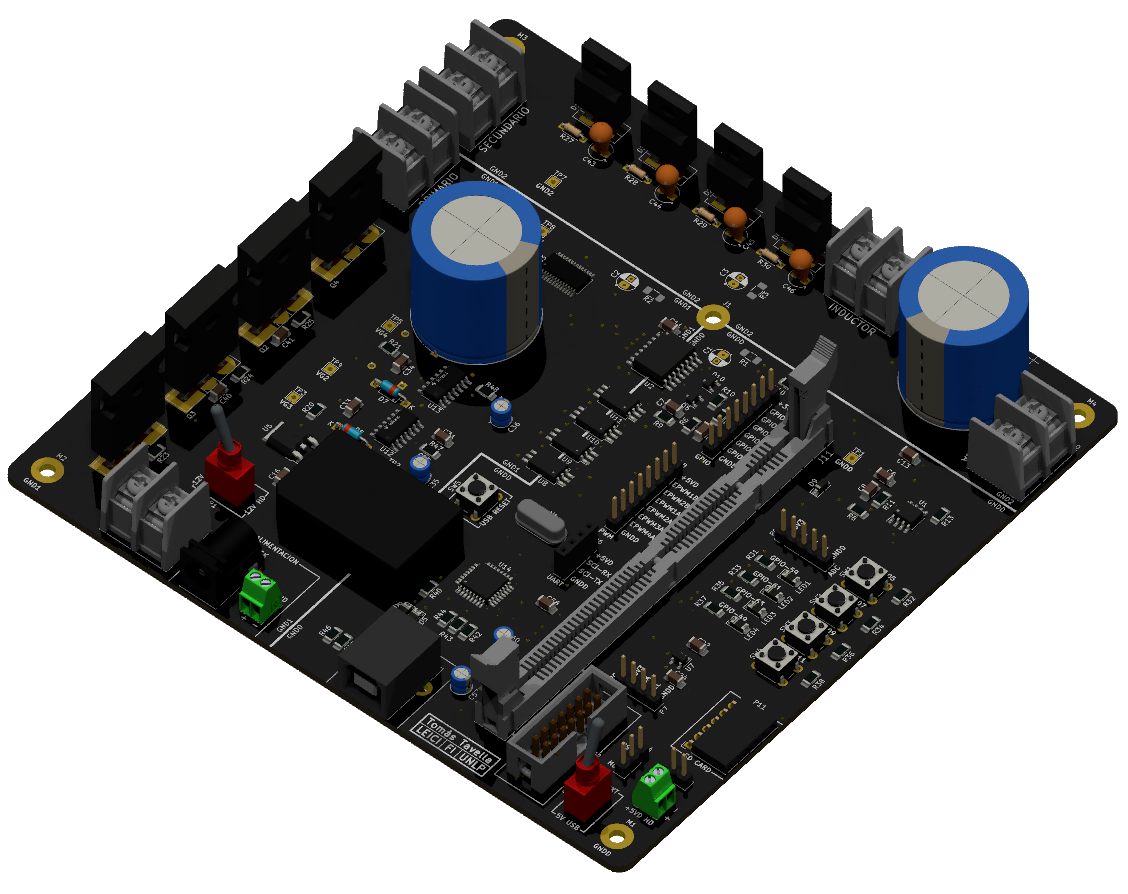
\includegraphics[scale=0.3]{Imagenes/PCB 3D Raytracing.png}
    \caption{Modelo tridimensional de la implementación en PCB de la plataforma con todos sus componentes, vista desde la parte superior.}
    \label{pcb_3d}
\end{figure}

Además de los componentes que se mencionaron o fueron mostrados en el proceso de diseño, existen otros componentes como conectores, borneras, pulsadores, LEDs y algunas resistencias y capacitores que se omitieron, ya que conforman únicamente detalles que incumben solamente a la implementación física. Teniendo en cuenta esto, el total de componentes discretos de la PCB llega a los 185. Se puede observar un modelo tridimensional de la placa final con todos sus componentes, generado por KiCad.\\

\subsection{Diseño de PCB}

\subsubsection{Dimensiones y Composición}

Dada la gran cantidad de componentes, muchos de montaje superficial, se decidió apuntar a un diseño de PCB {\Medium doble faz o doble capa}, ya que duplica la superficie disponible para posicionar componentes SMD, además de facilitar el trabajo de ruteo de las pistas de cobre que conectan los componentes,tema que se tratará en detalle más adelante.\\

En tanto a las dimensiones de la placa, desde el comienzo del proceso de implementación se buscó obtener una PCB lo más compacta posible, evitando colocar grandes componentes sobre la superficie de la placa. Es por este motivo que tanto el transformador de alta frecuencia como el inductor del filtro de salida $L_f$, que poseen bobinados y núcleos ferromagnéticos de grandes dimensiones, se colocan fuera de la placa, conectados mediante borneras de alta corriente. El diseño final de la placa, cuyo modelo 3D se observa en la figura \ref{pcb_3d}, resultó con una forma cuadrada de {\Medium 15 cm x 15 cm} aproximadamente, con una superfice total de cobre de {\Medium 450 cm\textsuperscript{2}} por ser doble capa.\\

El grosor total de la placa, con todas sus capas, es de {\Medium 1,6 mm}, y como se puede ver en la figura \ref{doble_capa}, consta de cinco capas distintas: dos capas de cobre, superior e inferior, de {\Medium 0,035 mm} cada una que contienen todas las pistas de la plaqueta; dos capas de mascara anti-estaño de {\Medium 0,01 mm} arriba de cada capa de cobre que facilitan el proceso de soldado; y un dieléctrico de {\Medium 1,51 mm de FR-4}, un laminado de resina epoxi reforzado con vidrio, que aisla las dos capas de cobre.\\

\begin{figure}[h]
    \centering
    
\includegraphics[scale=0.4]{Imagenes/Perfil Doble Capa.png}
    \caption{Corte transversal de una placa de circuito impreso doble capa, con mascara anti-estaño indicada en verde.}
    \label{doble_capa}
\end{figure}

Adicionalmente, en el diseño de la placa se utilizan orificios \textit{through-hole} y vías (perforaciones que unen dos pistas de cobre en distintas capas) de tipo {\Medium PTH}, del inglés \textit{Plated Through-Hole}, que consisten en orificios que atraviesan toda la PCB, cuyas paredes internas son cubiertas con una fina capa de cobre que las hace conductoras, que genera una conexión entre las pistas unidas por las vías u orificios THT.\\

Finalmente, entre las capas de cobre y las máscaras correspondientes se coloca una capa llamada {\Medium\textit{silkscreen}}, que contiene el texto de identificadores de componentes y otras líneas que ayudan a la hora de ubicar componentes en la placa. Para dibujar estas líneas se utiliza un material no conductor, por lo que pueden ponerse por encima de líneas de cobre.\\

\subsubsection{Asignación de Footprints}

Antes de comenzar a ubicar los componentes y definir la disposición general de la placa, se debe tomar la lista completa de estos componentes y asignarle a cada uno una \textit{footprint}. Las footprints son los patrones de \textit{pads} para componentes SMD y orificios para componentes THT que se imprimen en cobre sobre la capa correspondiente de la placa, y sobre los cuales se colocan los componentes correspondientes para ser luego soldados con estaño.\\

\begin{figure}[h]
    \centering
    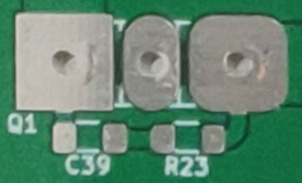
\includegraphics[scale=0.4]{Imagenes/Ejemplo Footprint.jpg}
    \caption{Ejemplo de footprint de un componente THT tipo TO-247, y dos componentes SMD tipo 1206.}
    \label{footprints}
\end{figure}

Con este fin se utilizan páginas tales como SnapEDA o UltraLibrarian, que poseen masivas bibliotecas gratuitas de modelos de componentes, footprints y modelos 3D, de utilidad cuando las bibliotecas incluidas con KiCad no contienen el componente que se necesita. Los circuitos integrados y otros componentes que se mencionaron en el capítulo anterior ya tienen su encapsulado, y por la tanto su footprint, definidas. Sin embargo, muchos componentes pasivos como resistencias, capacitores, diodos y LEDs que no fueron mencionados específicamente vienen en una variedad de empaquetados.\\

La mayor parte de estos componentes pasivos que se encuentran distribuidos sobre la placa se seleccionaron con empaquetados y footprints de montaje superficial de pequeños tamaños, la mayoría de tamaño 1206. Este código numérico indica sus dos dimensiones principales en centésimas de pulgada, que pasado al sistema métrico resulta de \SI[]{3}{\milli\meter} x \SI[]{1.5}{\milli\meter}.\\

\begin{figure}[h]
    \centering
    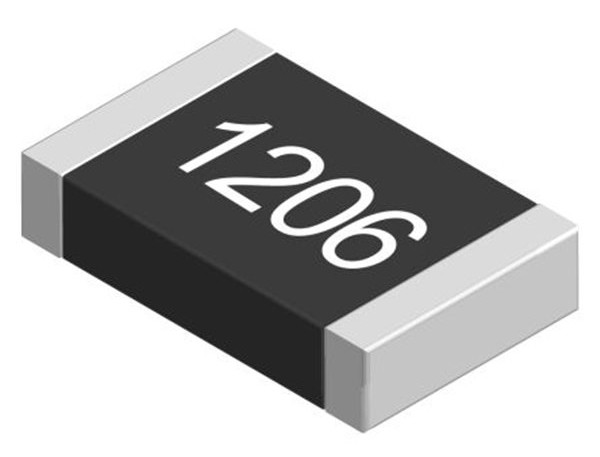
\includegraphics[scale=0.4]{Imagenes/1206.jpg}
    \caption{Modelo tridimensional de un resistor SMD 1206 estándar.}
    \label{smd1206}
\end{figure}

En algunos pocos casos se utilizan componentes pasivos de empaquetado distinto, como el encapsulado SMD 2512 (\SI[]{6.3}{\milli\meter} x \SI[]{3.2}{\milli\meter}) para la resistencia shunt del LM5056A, los encapsulados THT de distintos diámetros para algunos capacitores electrolíticos, entre otros. A continuación se presenta una lista con todas las distintas footprints/encapsulados utilizados en la PCB, separados entre SMD y THT.\\

\begin{multicols}{3}
    \begin{itemize}
        \item 1206 (SMD)
        \item 2512 (SMD)
        \item SOD-123 (SMD)
        \item SOT-23-3 (SMD)
        \item SOT-23-5 (SMD)
        \item SOIC-8 (SMD)
        \item SOIC-16W (SMD)
        \item HTSSOP-28 (SMD)
        \item TO-252-2 (SMD)
        \item SSO-6 (SMD)
        \item SO-14 (SMD)
        \item LQFP-32 (SMD)
        \item TO-220F-2 (THT)
        \item DO-35 (THT)
        \item Pin Header 2.54 mm (THT)
        \item USB-B (THT)
        \item TO-247-3 (THT)
        \item DIP-24 (THT)
        \item HC-18 (THT)
        \item DIMM-100 (THT)
        \item[\vspace{\fill}]       % Para que la segunda columna quede bien espaciada verticalmente con cantidad impar de elementos
    \end{itemize}
\end{multicols}

\subsubsection{Disposición de Componentes}

Para disponer los componentes dentro del área de la placa, se tomó como criterio principal la obtención del diseño más compacto posible. Sin embargo, siempre se debe dejar un espacio suficiente para poder soldar cómodamente todos los componentes, por lo que existe un límite en la cercanía entre componentes, en especial para componentes de grandes dimensiones tales como el capacitor del filtro de salida.\\

Además, también se tuvo que tener en cuenta la agrupación de componentes de acuerdo a su puesta a tierra, que en muchos casos va en detrimento de un diseño compacto. Esta agrupación resultó en algunos grandes espacios con baja densidad de componentes, particularmente en la zona de la tierra del secundario $GND_2$.\\

En tanto a las dos capas de cobre, la mayor parte de los componentes se encuentran concentrados en la capa superior, con la capa inferior relegada mayormente a componentes pasivos y de menor tamaño, como resistencias y capacitores SMD. Todos los componentes de interfaz con persona, como conectores, borneras, interruptores, pulasdores y LEDs se posicionaron en el frente de la placa por una cuestión de comodidad de operación.\\

\subsubsection{Trazado y Dimensionamiento de Pistas}

Una vez ordenados los componentes, separados apropiadamente según la puesta a tierra que le corresponde, se procedió a hacer el trazado o ruteo de las pistas de cobre que conectan los distintos componentes. Dado que las capas de cobre de la PCB son de grosor fijo, la capacidad de corriente de una pista se modifica únicamete aumentando el ancho de la misma.\\

\paragraph{Trazado de Pistas}

Para trazar la gran cantidad de pistas de cobre con las que cuenta la plataforma, se siguieron, siempre que fuese posible, algunas guías generales para su disposición: evitar generar antenas con pistas de cobre, cosa que se logra trazando pistas de cobre paralelas lo más cercanas entre sí que sea posible (ya que el efecto parásito de las antenas aumenta con la superficie encerrada); utilizar planos de tierra separados, para evitar inducir ruido en pistas de señal; evitar lo más posible agrupar líneas de señal con líneas de alta corriente; entre muchas otras.\textsuperscript{\cite{PCBLayout}}\\

Adicionalmente, dónde estuviera disponible se siguieron las recomendaciones de disposición en PCB de integrados particulares que se encontraran en sus hojas de datos (por ejemplo, para el aislador ISO7242C, la hoja de datos recomienda que debajo del dispositivo no exista ninguna pieza de cobre).\\

\paragraph{Cálculo de Ancho de Pista}

Todas las pistas de cobre en la PCB se dimensionaron según la ecuación establecida por la {\Medium norma IPC-2221}, que permite calcular el ancho $W$ (en \unit{\milli\metre}) necesario para una que una pista de cobre de grosor $H$ (en \unit{\milli\metre}) con una corriente circulante $I$ (en \unit{\ampere}) no eleve su temperatura más de $\Delta T$ grados centígrados.

\begin{equation}\label{eq:IPC2221}
    I = \num{0.048}\cdot (\Delta T)^{\num{0.44}}\cdot (\num{1550}\cdot W\cdot H)^{\num{0.725}}
\end{equation}

En este caso, el grosor $H$ de las pistas es fijo de \SI[]{0.035}[]{\milli\metre} con una máxima elevación de temperatura $\Delta T$ de \SI[]{20}[]{\celsius}, aunque sería preferible un valor más conservador de \SI[]{10}{\celsius}. Entonces, reemplazando la corriente por el máximo valor de corriente que puede circular por una pista, se puede despejar su ancho mínimo $W$ en \unit{\milli\metre}.\\

\subparagraph{Pistas Estándar}

Como ancho de pista estándar se eligió un valor de {\Medium 0,25 mm}. Una pista de este ancho necesita casi \SI[]{700}{\milli\ampere} de corriente para elevar su temperatura \SI[]{5}{\celsius} sobre la temperatura ambiente, según lo calculado con la ecuación \ref{eq:IPC2221}, por lo que es apta para ser usada en cualquier línea de cobre que no maneje elevadas potencias.\\

\subparagraph{Pistas de Alta Corriente}

Para las pistas que forman parte de los circuitos del primario y secundario del convertidor puente, se requieren pistas de mucho mayor ancho, dadas la elevadas circulaciones de corriente. En el secundario pueden llegar a circular corrientes constantes de hasta \SI{4}{\ampere}, mientras que en los circuitos del primario, que son de menor tensión, puede llegar a manejar corrientes no transitorias de hasta \SI{10}{\ampere}.\\

En el caso del {\Medium primario}, dado el muy elevado valor de corriente, se eligió un {\Medium ancho de pista de 5 mm}, que resulta en una elevación de temperatura $\Delta T$ de alrededor de \SI[]{18}{\celsius} para el máximo valor posible de corriente. En este caso se tuvo que seleccionar un ancho de pista ajustado, casi llegando a la máxima $\Delta T$, principalmente por limitaciones de espacio.\\

Para el {\Medium secundario}, el valor de corriente es menor a la mitad del máximo, por lo que su ancho de pista se disminuyó proporcionalmente hasta un {\Medium ancho de 2 mm}. Sin embargo, como la relación establecida por la norma IPC-2221 no es lineal, este valor de $W$ resulta mucho mas holgado, con una elevación menor a \SI{11}{\celsius} para corrientes de \SI[]{4}{\ampere}.\\

Siempre se intenta mantener las pistas de altas corrientes (o que transportan señales susceptibles a distorsión e interferencia), en la misma capa de cobre. En caso de no ser posible, ya sea por componentes que se interponen en el camino u otras razones, se utilizan \textit{vías PTH} que permiten conectar eléctricamente pistas en distintas capas de cobre.\\

\paragraph{Planos de Tierra}

En el caso de las tres puestas a tierra, se utilizó la funcionalidad \textit{fill zone} o rellenar zona en lugar de utilizar pistas individuales. Esta funcionalidad permite elegir una zona de una o varias capas de cobre y rellenarla con cobre en todas las partes en las que no haya una pista preexistente, para luego conectar todos los terminales correspondientes a una de las tierras a este plano de cobre. Su principal beneficio se encuentra en la disipación térmica del calor generado por las altas corrientes, ya que en las tierras circulan todas las corrientes de los dispositivos combinadas. Además, esta configuración mejora la inmunidad electromagnética del sistema, y simplifica el procedimiento de trazado de las pistas.\\

\begin{figure}[h]
    \centering
    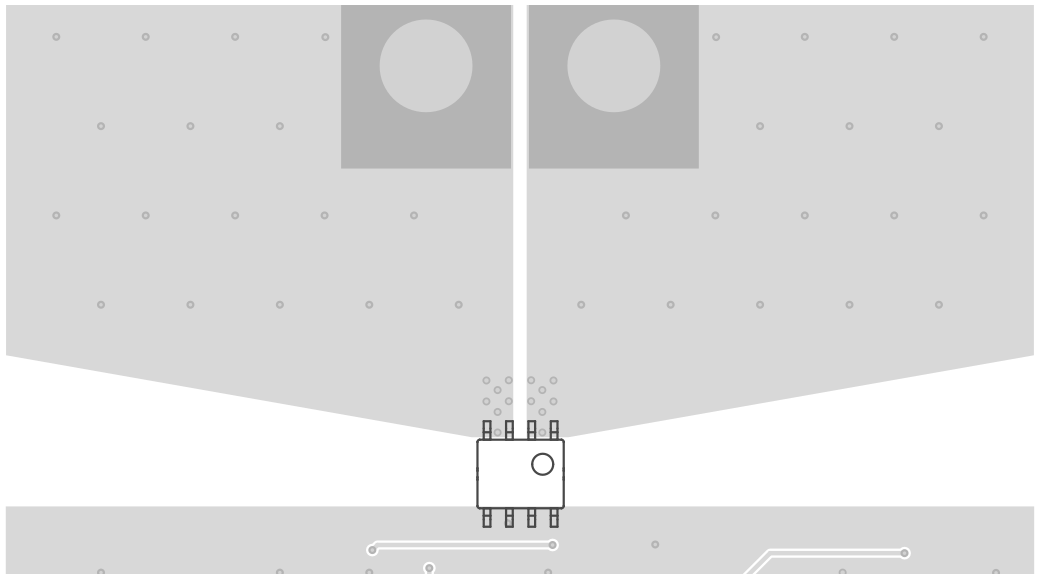
\includegraphics[scale=0.25]{Imagenes/Planos TMCS1100.png}
    \caption{Layout de conexión recomendado para el sensor de efecto Hall TMCS1100A4, utilizando planos de cobre.\textsuperscript{\cite{TMCS1100}}}
    \label{plano_tierra_tmcs}
\end{figure}

En algunos casos se utilizó esta funcionalidad del programa para otros planos
no conectados a tierra, en particular para planos de alimentación de \SI[]{5}{\volt} del lado digital; y para los pines de sensado de corriente por efecto Hall del TMCS1100A4, según indicado en la hoja de datos del fabricante, cómo se ve en la figura \ref{plano_tierra_tmcs}.\\

\subsubsection{Fabricación y Resultado}

Para la fabricación de la placa de circuito impreso que se diseñó, se evaluaron varias opciones de fabricantes locales, finalmente seleccionando al fabricante nacional {\Medium Mayer Circuitos Impresos}, radicado en Capital Federal. Una vez seleccionado, se tomaron los dates de estándares de fabricación disponibles en la página web, que indican las tolerancias de fabricación, y se ingresaron a una interfaz del diseñador de PCB de KiCad llamado \textit{Design Rules Checker}.\\

En base a los datos ingresados, se ejecuta esta herramienta que compara las medidas mínimas ingresadas con las medidas del diseño, e indica los lugares que se encuentran por debajo de la tolerancia mínima. Con esta herramienta se corrigieron múltiples errores y componentes muy cercanos a las tolerancias mínimas, como por ejemplo algunas vías que estaban por debajo del diámetro mínimo.\\

Con estos errores corregidos y el diseño verificado, se generaron los archivos \textit{gerber} y \textit{drill} y fueron envíados por correo electrónico al fabricante. Como no era posible fabricar una única placa, se encargó la mínima cantidad posible: un lote variable de entre tres y cinco unidades, con un tiempo estimado de fabricación y envío de un mes.\\

\begin{figure}[h]
    \centering
    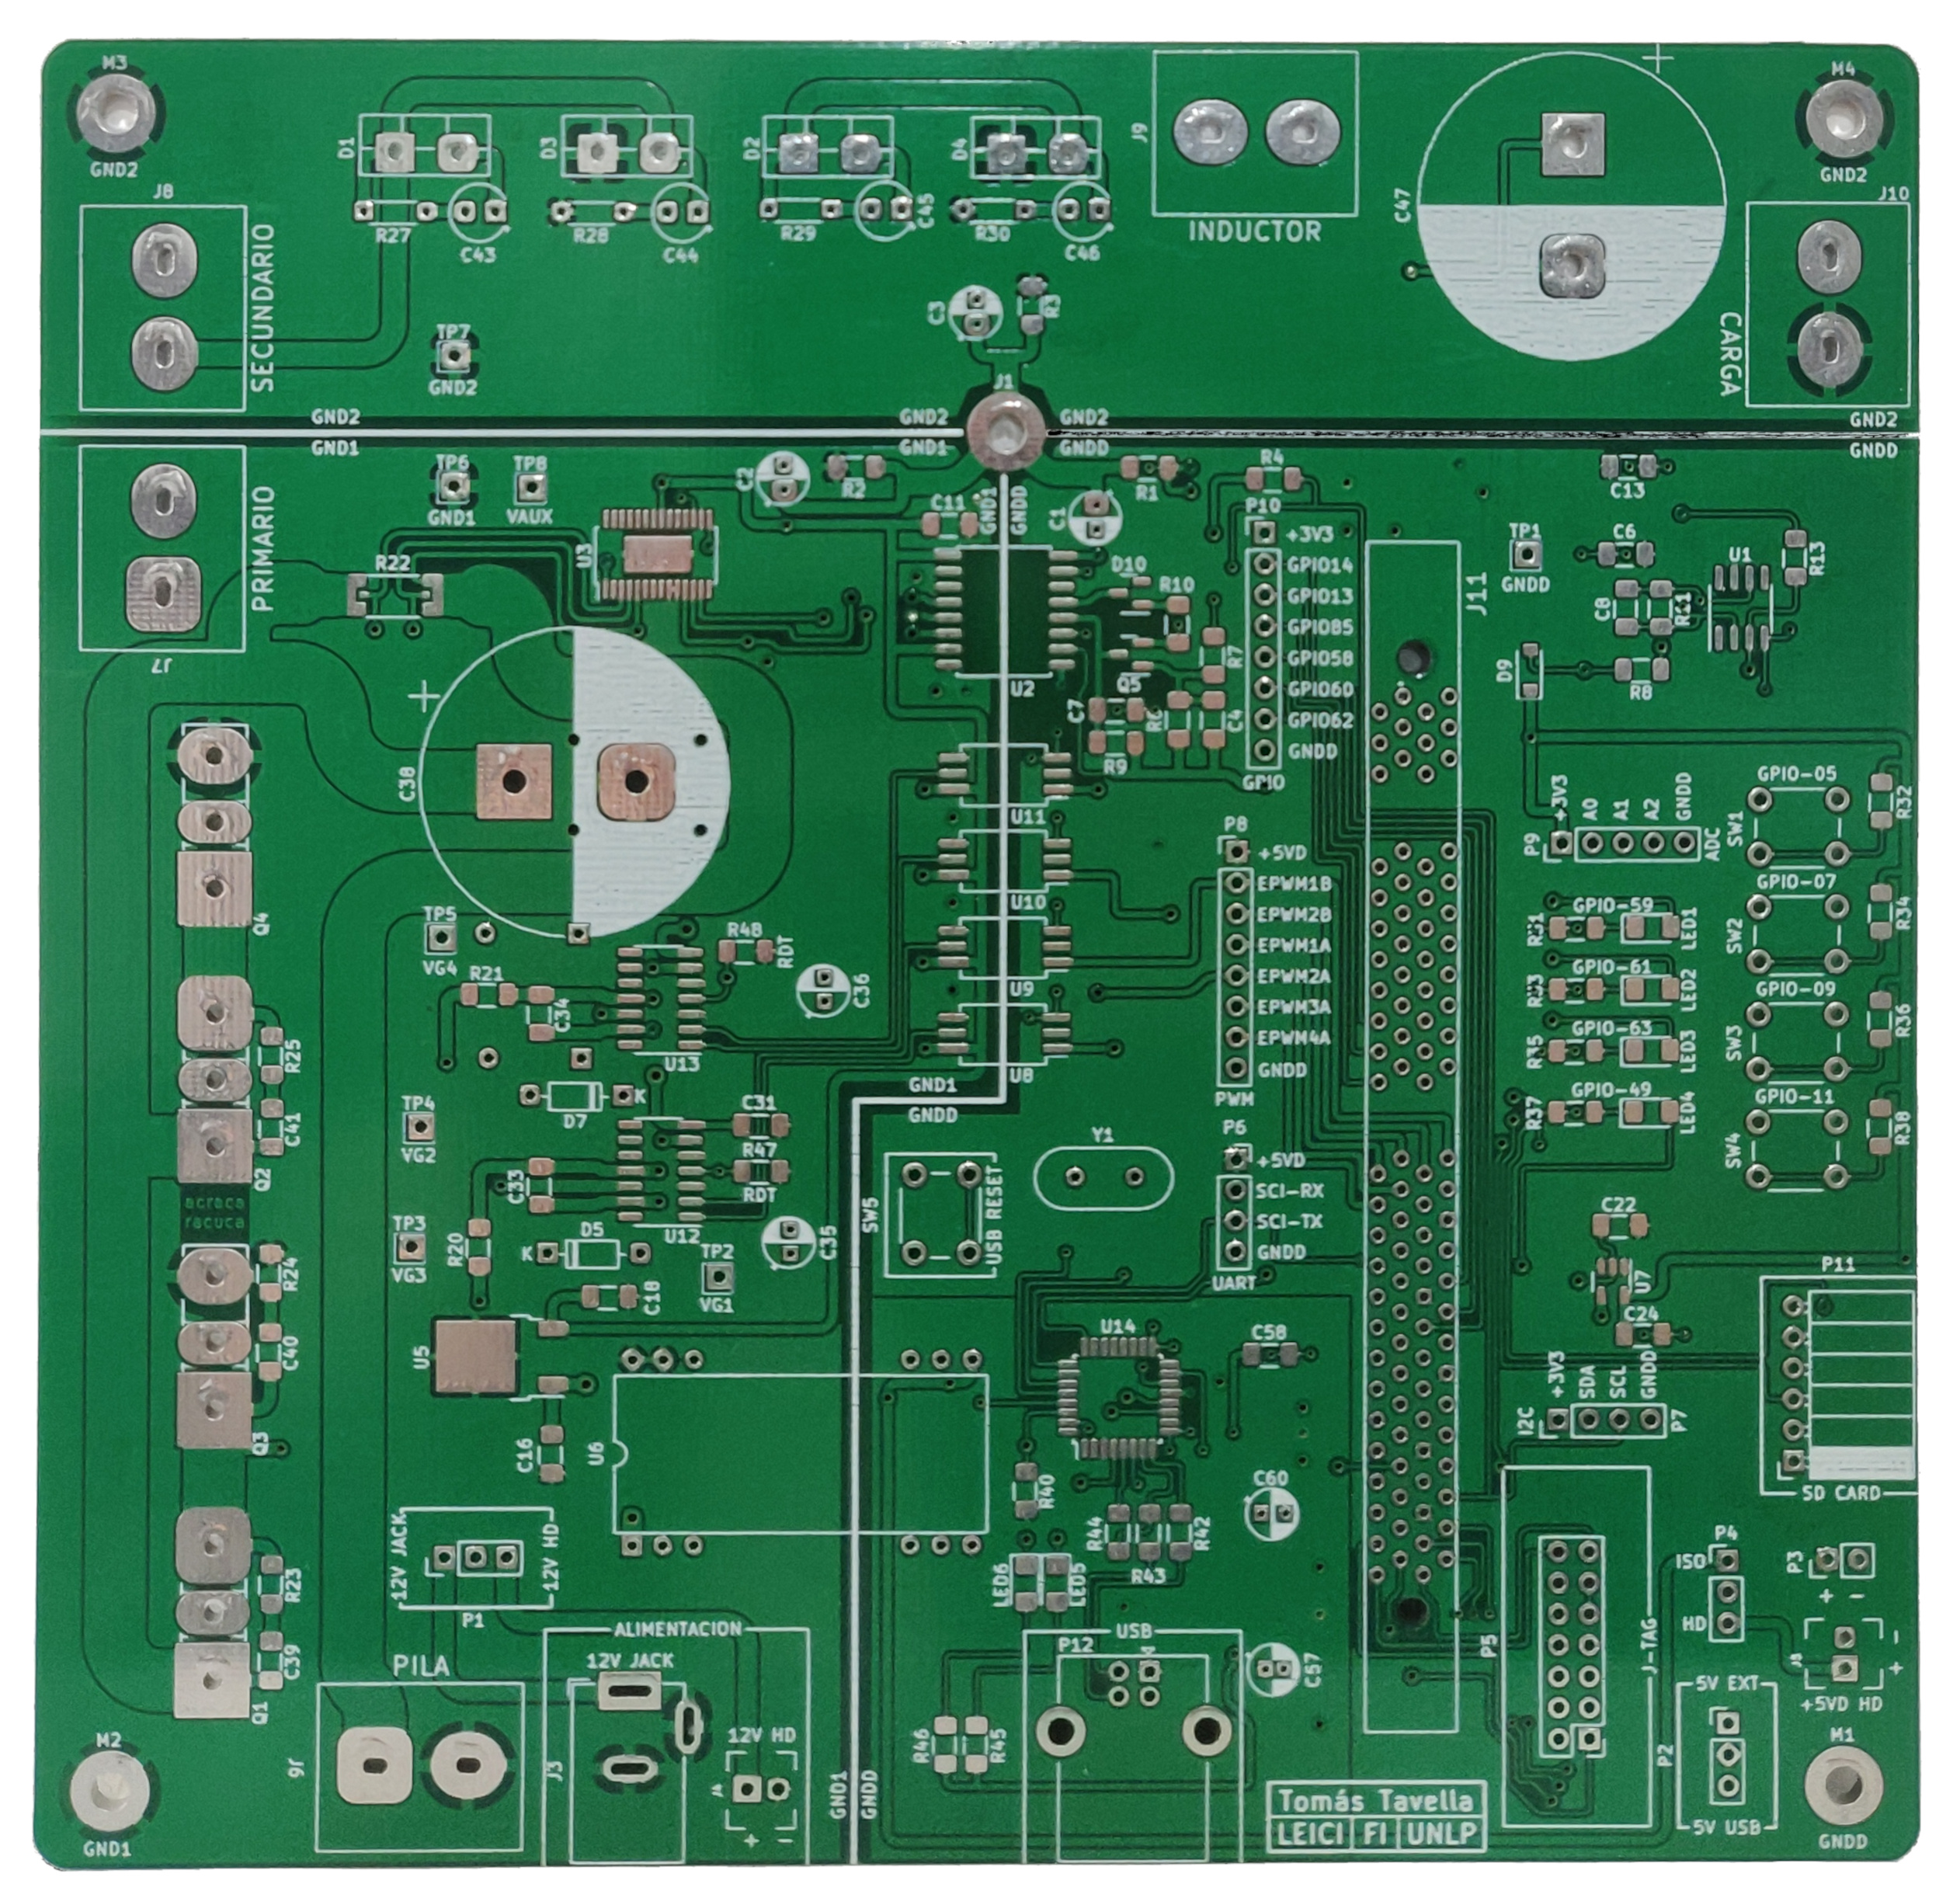
\includegraphics[scale=0.13]{Imagenes/Placa Fisica.jpg}
    \caption{Capa superior de la PCB fabricada por la empresa Mayer Circuitos Impresos, sin componentes soldados.}
    \label{placa_fisica}
\end{figure}

En la figura \ref{placa_fisica} se puede observar una fotografía de la capa de cobre superior de la placa resultante fabricada por Mayer Circuitos impresos. El resultado cumplió con las expectativas de calidad, y no se encontró ningún defecto de fabricación en ninguna de las copias recibidas.\\

\newpage

\subsection{Soldado de Componentes}

Una vez que las placas fabricadas arribaron al laboratorio como en la figura \ref{placa_fisica} y todos los componentes de la plataforma se encontraban disponibles en el laboratorio, se comenzó el proceso de soldar el total de 180+ componentes discretos a la placa, que se completó en un marco de tiempo de aproximadamente tres semanas.\\

\begin{figure}[h]
    \centering
    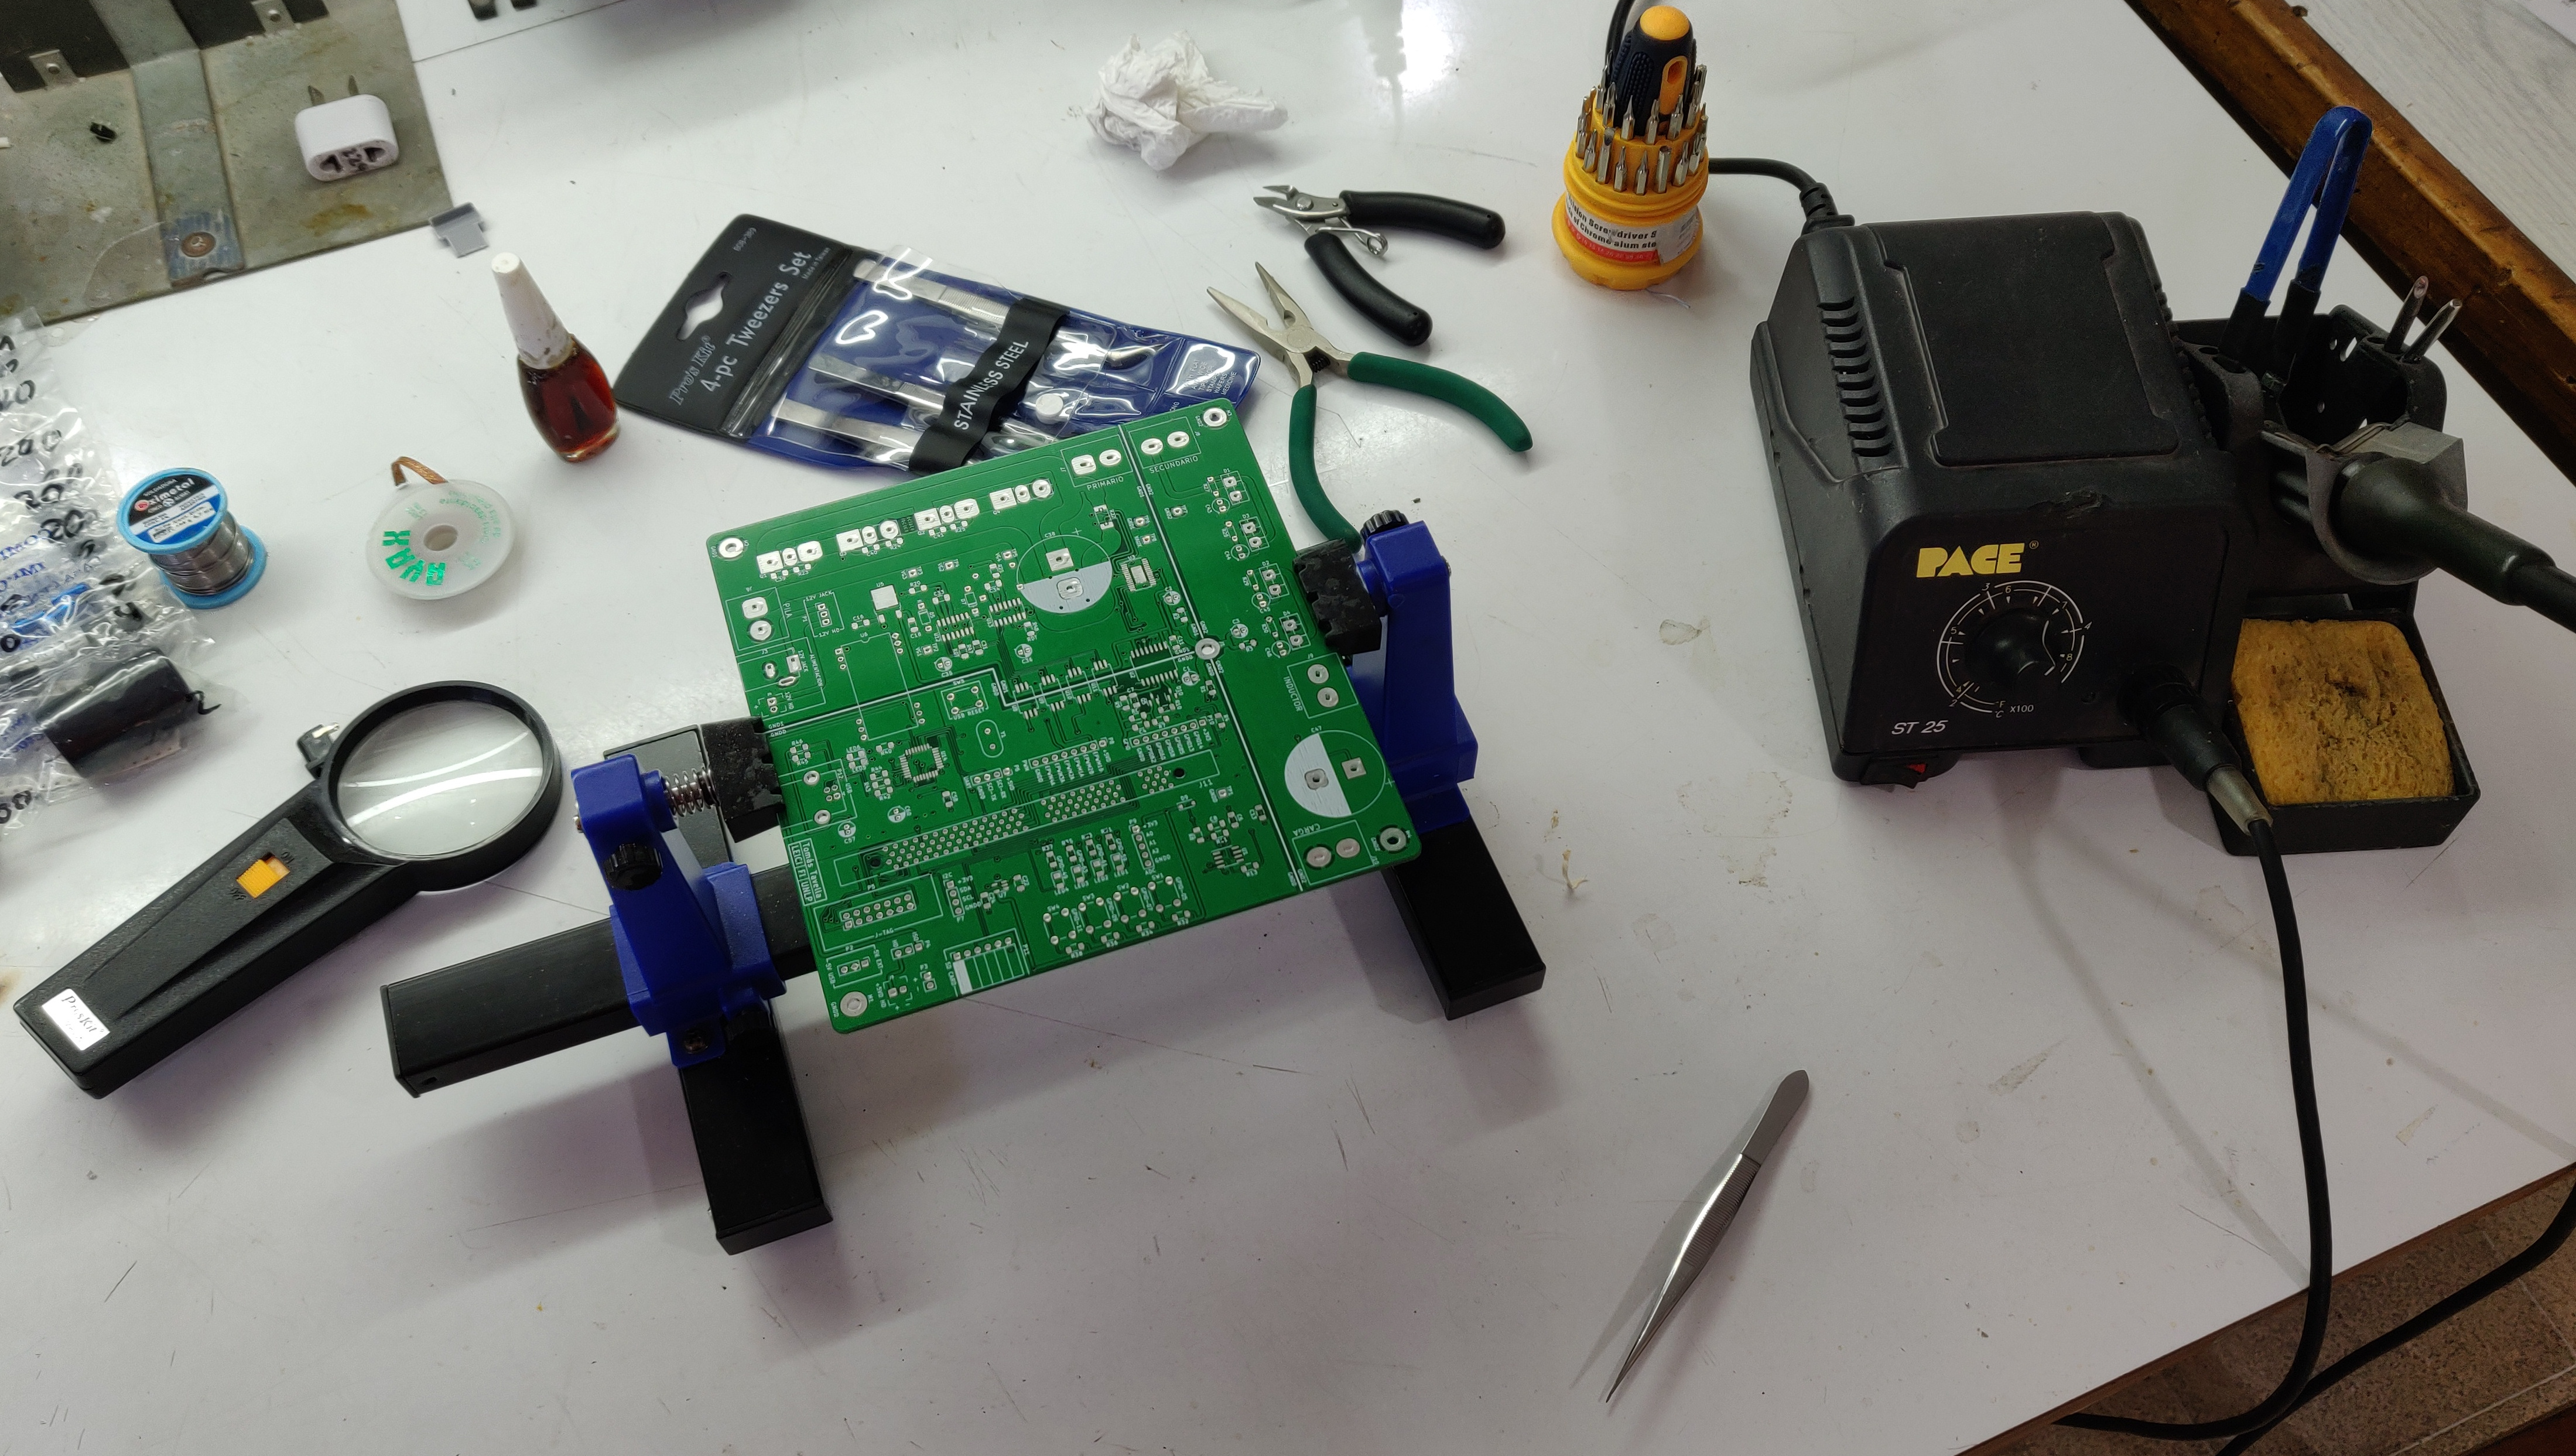
\includegraphics[scale=0.09]{Imagenes/Soldado.jpg}
    \caption{Zona de trabajo dónde se realizó el soldado de los componentes. A la derecha se puede observar la estación de soldado de temperatura regulable.}
    \label{soldado}
\end{figure}

Con asistencia del director del proyecto se aprendieron las nociones básicas de soldado de componentes SMD, y se completó todo el proceso sin mayores inconvenientes. Se comenzó soldando todos los componentes necesarios para evaluar el correcto funcionamiento del circuito driver y la excitación PWM, que incluyen los dos drivers medio puente de 2ED21834-S06J y todos su circuito auxiliar, los optoacopladores ACPL-P480 para aislar el DSC, el conector \textit{barrel} para la alimentación externa y el regulador lineal LM7805 para alimentar los optoacopladores.\\

Luego se continuó soldando el resto de los componentes, dejando los de mayores dimensiones físicas, en particular los capacitores de entrada y salida del convertidor, para el final del proceso, de manera que no estorben para la colocación de otros componentes.\\

El único componente que presento alguna dificultad al soldar fue el sensor LM5056A, cuyo empaquetado HTSSOP-28 cuenta con un pad encontrado en la parte inferior. En este caso, este pad es simplemente una conexión a tierra y cumple el único propósito de mejorar la capacidad de disipación térmica del dispositivo. Como no se cuenta con el equipo apropiado para soldar esta conexión, se utilizó una pasta térmica no conductora para al menos conseguir algín nivel de transferencia de calor del sensor al plano de tierra.\\

\newpage

\subsection{Contratiempos}

\lipsum[1]\\

\subsubsection{Placa Adaptadora}

\lipsum[2]\\

\newpage

\subsection{Resumen}

En este capítulo se detalló el proceso mediante el cual se pasó de un diseño circuital teórico para la plataforma de evaluación de sistemas híbridos obtenido en el capítulo anterior, a una PCB real de más de 180 componentes discretos que implementa el sistema.\\

Primero se trató el diseño de la PCB en el \textit{PCB Editor} de KiCad partiendo del circuito diseñado, eligiendo footprints para cada componente, ordenándolos de manera lógica en el área física de la placa, trazando y dimensionado las pistas de cobre que interconectan cada componente. Con el diseño finalizado, se enviaron los archivos de fabricación a una fábrica local de circuitos impresos.\\

Una vez obtenidas las placas producidas por el fabricante de acuerdo a las especificaciones del diseño, se procedió a soldar cada uno de los componentes, así obteniendo una placa finalizada y funcional. Además, se detallaron los inconvenientes importantes que surgieron y se debieron resolver a lo largo del proceso.\\

Con los resultados de este capítulo, la plataforma se encuentra lista para los ensayos que verificarán su funcionamiento correcto en el siguiente capítulo.\\

\afterpage{\blankpage}\newpage
%\newpage